\chapter{適用例}
\label{cha:Indication}

本研究では、既存ツールの問題を解決するために、自然言語仕様書から、
クラス、インスタンス変数定義、操作定義を記述したVDM++仕様書を生成する手法を提案し、
既存ツールに適用することでVGMLを開発した。

適用例では、VGMLに自然言語仕様書を適用することで、クラス、型定義、定数定義、インスタンス変数定義、操作定義を記述したVDM++仕様書を生成できること、
かつ、生成したVDM++仕様書の構文が正しいことを確認する。また、VGMLが教師データの自然言語仕様書と異なる自然言語仕様書に対応できることを確認する。

\section{教師データの自然言語仕様書と同じ自然言語仕様書の適用}
\label{sec:generate_vdm}

VGMLに、Microsoft社のwordで記述した自然言語仕様書「インターンシップ評定書・オンライン提出システム」(付録A.参照)を適用し、VDM++仕様書を生成する。
以降、自然言語仕様書「インターンシップ評定書・オンライン提出システム」を、仕様書Aと表現する。

この適用例では、学習済みモデルを生成するために使用した教師データの自然言語仕様書と同じ自然言語仕様書をVGMLに適用することによって、
VGMLが、VDM++仕様書のクラス、型定義、定数定義、インスタンス変数定義、操作定義を生成できること、かつ、生成したVDM++仕様書の構文が正しいことを確認する。

VGMLに仕様書Aを適用した結果、6つのファイルを生成した。
VGMLが仕様書Aを基に生成した6つのファイルを、図\ref{fig:indication_vdm1}-図\ref{fig:indication_vdm6}に示す。
図\ref{fig:indication_vdm1}-図\ref{fig:indication_vdm6}は、VDM++ Toolbox\cite{Tools}での出力の画面である。

\begin{figure}[p]
    \begin{center}
    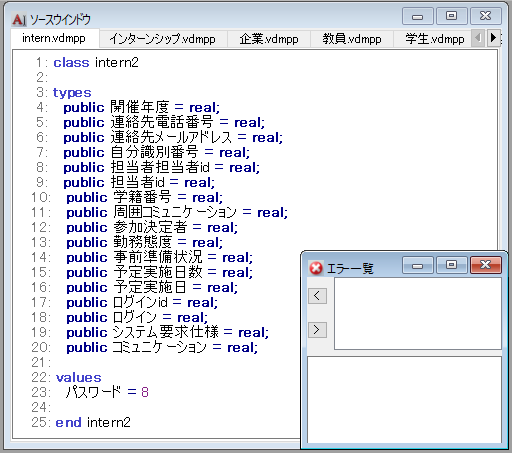
\includegraphics[width=300]{image/indication_vdm1.PNG}
    \caption{VGMLが仕様書Aを基に生成したファイル1}
    \label{fig:indication_vdm1}
    \end{center}
\end{figure}

\begin{figure}[p]
    \begin{center}
    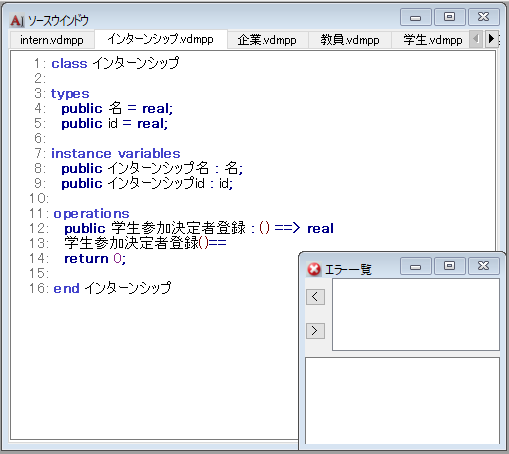
\includegraphics[width=300]{image/indication_vdm2.PNG}
    \caption{VGMLが仕様書Aを基に生成したファイル2}
    \label{fig:indication_vdm2}
    \end{center}
\end{figure}

\begin{figure}[p]
    \begin{center}
    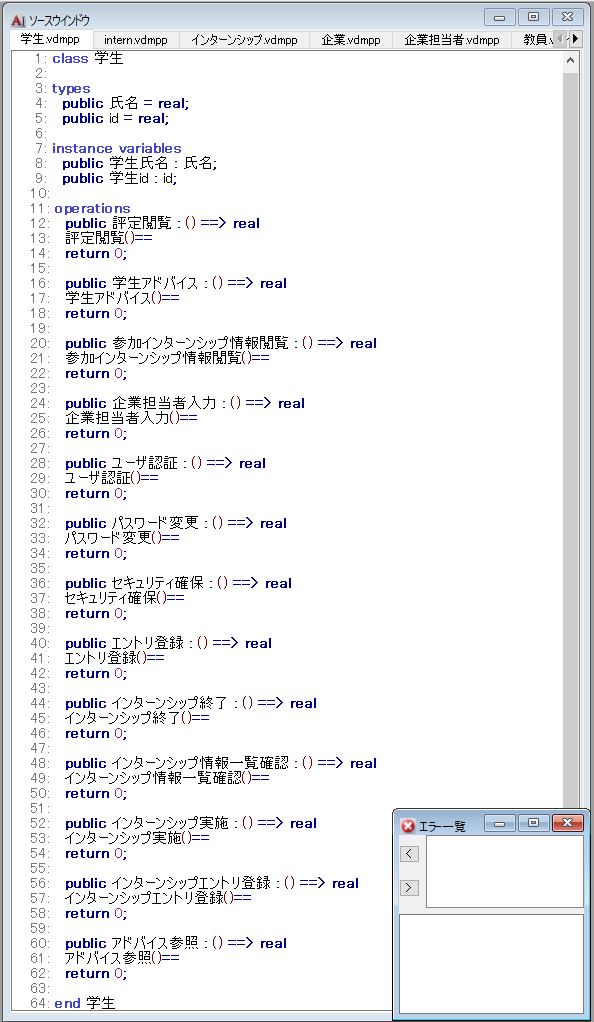
\includegraphics[width=300]{image/indication_vdm3.PNG}
    \caption{VGMLが仕様書Aを基に生成したファイル3}
    \label{fig:indication_vdm3}
    \end{center}
\end{figure}

\begin{figure}[tp]
    \begin{center}
    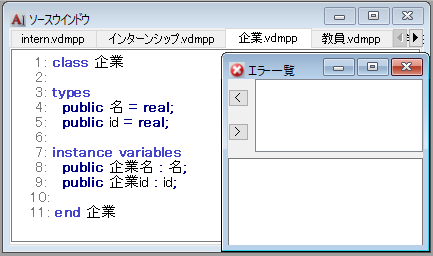
\includegraphics[width=300]{image/indication_vdm4.PNG}
    \caption{VGMLが仕様書Aを基に生成したファイル4}
    \label{fig:indication_vdm4}
    \end{center}
\end{figure}

\begin{figure}[tp]
    \begin{center}
    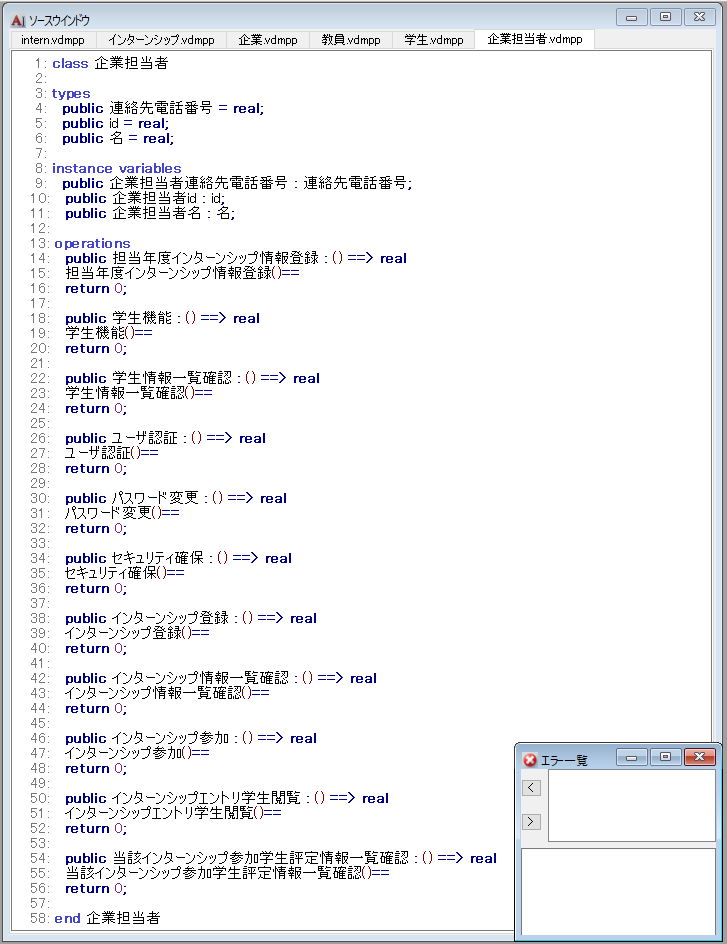
\includegraphics[width=300]{image/indication_vdm5.PNG}
    \caption{VGMLが仕様書Aを基に生成したファイル5}
    \label{fig:indication_vdm1}
    \end{center}
\end{figure}

\begin{figure}[tp]
    \begin{center}
    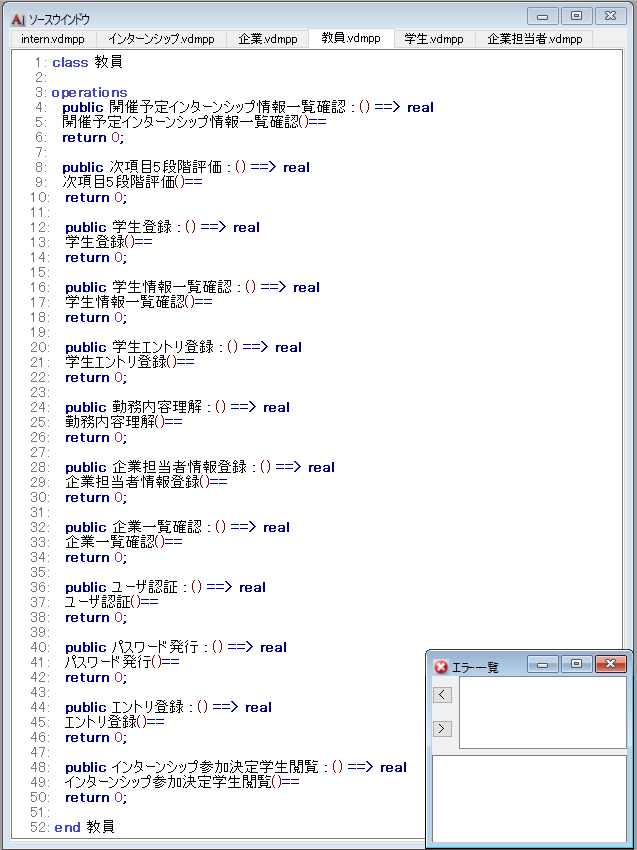
\includegraphics[width=300]{image/indication_vdm6.PNG}
    \caption{VGMLが仕様書Aを基に生成したファイル6}
    \label{fig:indication_vdm6}
    \end{center}
\end{figure}

構文、および、タイプチェッカーを備えたVDM++ Toolboxは、生成したVDM++仕様書に対して警告を表示しなかった。
このことから、VGMLに自然言語仕様書を適用することにより、
クラス、型定義、定数定義、インスタンス変数定義、操作定義を記述したVDM++仕様書を生成できること、
かつ、生成したVDM++仕様書の構文が正しいことを確認した。

\section{教師データの自然言語仕様書と異なる自然言語仕様書の適用}
\label{sec:different_generate_vdm}

VGMLに、pdfで記述した「ETロボコン2020競技規約」\cite{ET_robo}を適用し、VDM++仕様書を生成する。
また、学習済みモデルについては、\ref{sec:vgml_train_model}節で仕様書Aを基に生成した学習済みモデルを使用する。
付録B.に、「ETロボコン2020競技規約」の自然言語仕様書の$4~13$ページ、および、$24~31$ページを示す。
なお、今回対象としなかった$1~3$ページは、目次および仕様書を読むための項目であったため対象から外した。
さらに、「ETロボコン2020」の競技は、3つのクラスに別れており、今回はアドバンストクラスについての自然言語仕様書である$24~31$ページを対象とした。
以降、「ETロボコン2020競技規約」の$24~31$ページを、仕様書Bと表現する。

この適用例では、学習済みモデルを生成するために使用した教師データの自然言語仕様書と異なる自然言語仕様書をVGMLに適用することによって、
VGMLが、教師データの自然言語仕様書と異なる自然言語仕様書に対しても、
VDM++仕様書のクラス、型定義、定数定義、インスタンス変数定義、操作定義を生成できること、かつ、生成したVDM++仕様書の構文が正しいことを確認する。

VGMLに仕様書Bを適用した結果、6つのファイルを生成した。
VGMLが仕様書Bを基に生成した6つのファイルを、図\ref{fig:indicationB_vdm1}-図\ref{fig:indicationB_vdm6}に示す。
図\ref{fig:indicationB_vdm1}-図\ref{fig:indicationB_vdm6}は、VDM++ Toolbox\cite{Tools}での出力の画面である。
構文、および、タイプチェッカーを備えたVDM++ Toolboxは、生成したVDM++仕様書に対して警告を表示しなかった。

\begin{figure}[p]
    \begin{center}
    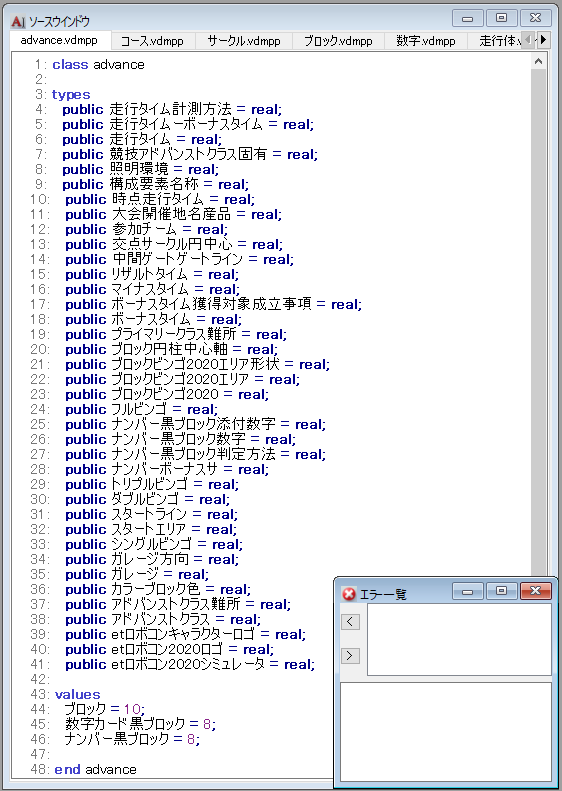
\includegraphics[width=300]{image/indicationB_vdm1.PNG}
    \caption{VGMLが仕様書Bを基に生成したファイル1}
    \label{fig:indicationB_vdm1}
    \end{center}
\end{figure}

\begin{figure}[p]
    \begin{center}
    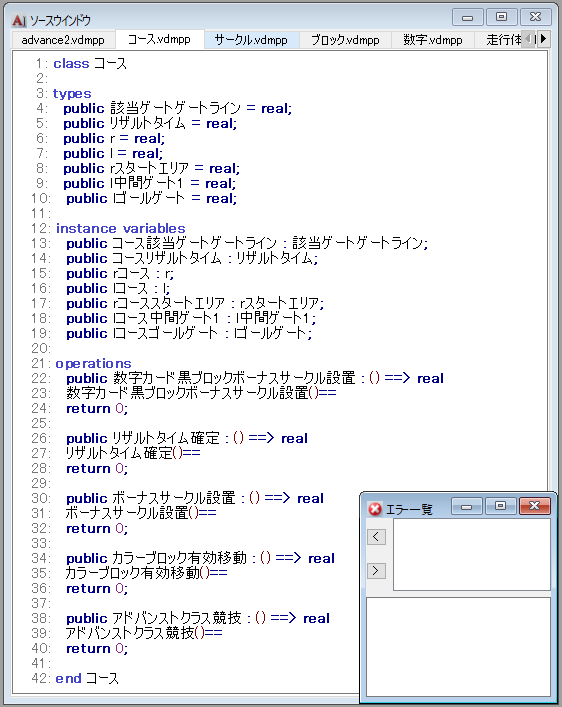
\includegraphics[width=300]{image/indicationB_vdm2.PNG}
    \caption{VGMLが仕様書Bを基に生成したファイル2}
    \label{fig:indicationB_vdm2}
    \end{center}
\end{figure}

\begin{figure}[p]
    \begin{center}
    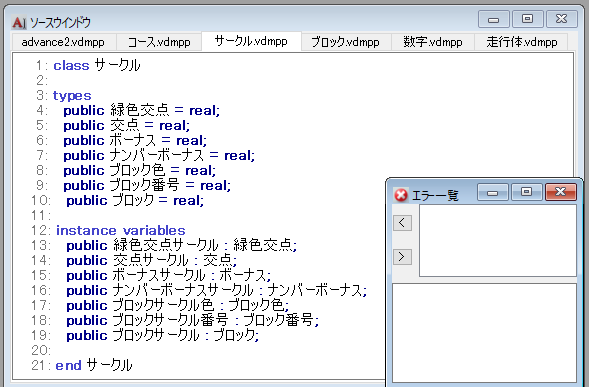
\includegraphics[width=300]{image/indicationB_vdm3.PNG}
    \caption{VGMLが仕様書Bを基に生成したファイル3}
    \label{fig:indicationB_vdm3}
    \end{center}
\end{figure}

\begin{figure}[tp]
    \begin{center}
    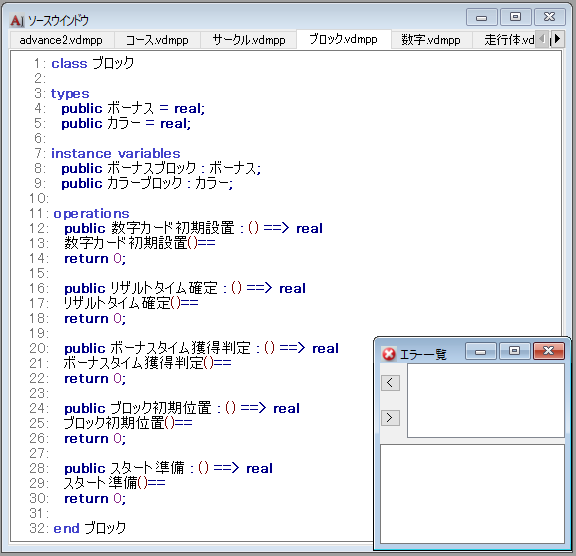
\includegraphics[width=300]{image/indicationB_vdm4.PNG}
    \caption{VGMLが仕様書Bを基に生成したファイル4}
    \label{fig:indicationB_vdm4}
    \end{center}
\end{figure}

\begin{figure}[tp]
    \begin{center}
    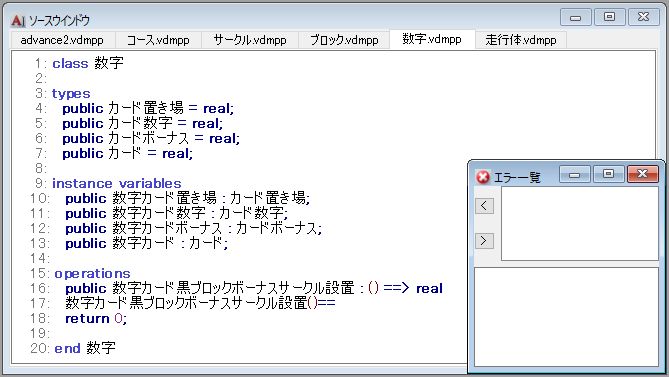
\includegraphics[width=300]{image/indicationB_vdm5.PNG}
    \caption{VGMLが仕様書Bを基に生成したファイル5}
    \label{fig:indicationB_vdm5}
    \end{center}
\end{figure}

\begin{figure}[tp]
    \begin{center}
    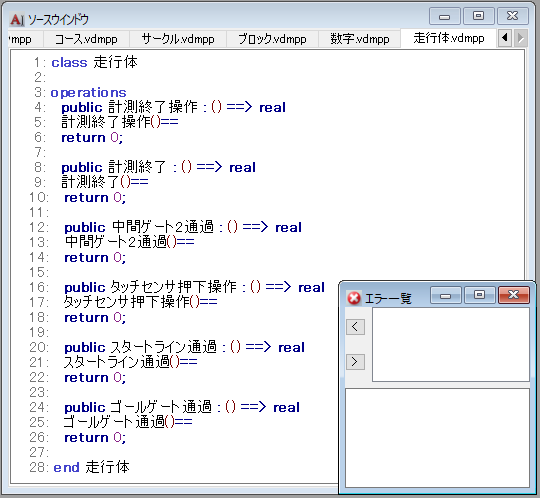
\includegraphics[width=300]{image/indicationB_vdm6.PNG}
    \caption{VGMLが仕様書Bを基に生成したファイル6}
    \label{fig:indicationB_vdm6}
    \end{center}
\end{figure}

このことから、VGMLに学習済みモデルを生成するために使用した教師データの自然言語仕様書と異なる自然言語仕様書を適用することにより、
学習済みモデルが教師データの自然言語仕様書と異なる自然言語仕様書に対しても、
VDM++仕様書のクラス、型定義、定数定義、インスタンス変数定義を生成できること、
かつ、生成したVDM++仕様書の構文が正しいことを確認した。

以上、\ref{sec:generate_vdm}節と\ref{sec:different_generate_vdm}節の適用結果により、VGMLが
VDM++仕様書のクラス、型定義、定数定義、インスタンス変数定義、操作定義を生成できること、かつ、生成したVDM++仕様書の構文が正しいことを確認した。